%!TEX root = /Users/velrok/Dropbox/TheoInf Seminar/Ausarbeitung/Main.tex
\section{Ähnlichkeitstheorie} % (fold)
\label{sub:Aehnlichkeitstheorie}

Die Ähnlichkeitstheorie besagt, das sich die Eigenschaften einer Modal-Logik in der Relation der entsprechenden Kripkestrucktur widerspiegeln und vis versa. 
Dies schafft einen neuen Zugang zum Design von Modal-Logiken. 
In manchen Fällen mag es einfacher sein in den notwendigen Eigenschaften in Form von Formel-Schemata zu denken, in anderen ist es evtl. einfacher das Problem über die Relation zu verstehen. 
Im Folgenden wird gezeigt, wie die einzelnen Eigenschaften mit der Kripke-Struktur-Relation zusammen hängen.


\paragraph{Zusammenhang zwischen der Relation $R$ und den validen \formelSchemata}

Wir haben in \Abs{festlegung_von_attibuten_mit_R} den Zusammenhang zwischen der Transitivität von $R$ und der Validität der Formel \vierFormel durch die Intuition begründet, dass die \emph{positive Introspektion} gilt.
Es wird nun gezeigt, dass sich dieser Zusammenhang mathematisch beweisen lässt.
Dazu muss zunächst der Begriff \emph{Frame} eingeführt werden:

\begin{definition}
	\label{def:frame}
	Ein Frame $\Fancy{F} = (W,R)$ ist eine Menge von Welten $W$ und eine binäre Relation $R$ auf $W$.
	\cite[S.322]{huth2004logic}
\end{definition}

\emph{Frames} kann man sich also als \KS ohne \emph{Labeling-Funktion} vorstellen.
Damit beschreiben sie die selbe Struktur, jedoch unabhängig von der Konkreten Wissensbasis, sprich den geltenden Facken in jeder Welt.
Damit übernehmen sie in Kripke-Strukturen die selbe Rolle wie \formelSchemata in \MLFn .

\begin{definition}
	\label{def:frame_erfuellt}
	Ein Frame $\Fancy{F}$ erfüllt eine modal logische Formal $\psi$, wenn für jede \fachwort{Labelfunktion} $L: W \rightarrow \Fancy{P}(Atome)$ und jedes $w \in W$, es der Fall ist, dass $\Fancy{M},w \vDash \psi$ gilt. $\Fancy{M}$ ist das Model: $\Fancy{M} = (W,R,L)$.
	In diesem Falle schreiben wir $\Fancy{F} \vDash \psi$.
	\cite[S.322f]{huth2004logic}
\end{definition}

Wenn ein Frame eine Formel erfüllt erfüllt es auch das entsprechende Schema. 

\begin{example}
	Das Beispiel-Frame auf \Abb{Kripke02} erfüllt die \TFormel.
	Um das zu beweisen muss man zeigen, dass jede Welt mit beliebiger Labeling-Funktion die Bedingung: wenn $x \VDash \Box p$ der Fall ist, dann gilt auch $x \VDash p$.
	Betrachten wie nun eine beliebige Welt $x \in W$ und setzen $x \VDash \Box p$, dann folgt aufgrund der Tatsache dass $R(x,x)$ gilt und der Regel für $\Box$ aus der \Def{reasoning}, dass $x \VDash p$ der Falls ein muss.
	Den $x$ zeigt auf sich selbst und ist damit in den von $x$ erreichbaren Welten enthalten

	\begin{figure}[h!]
		\label{fig:Kripke02}
		\centering
		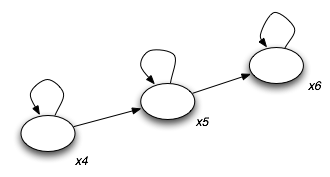
\includegraphics[width=10cm]{Images/Kripke02}
		\caption{Beispielframe}
	\end{figure}

	Da ein \emph{Frame} keine Annahme über eine konkrete Labeling-Funktion macht und wir gerade nachgewiesen haben, dass $\Box p \rightarrow p$ gilt, ist auch \TFormel der Fall.
	
	Die \vierFormel wird hingegen nicht erfüllt.
	Das Model in \Abb{Kripke03} beweist dies durch ein Gegenbeispiel.

	\begin{figure}[h!]
		\label{fig:Kripke03}
		\centering
		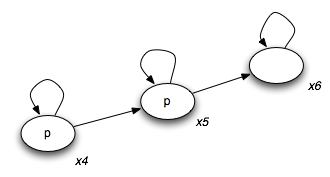
\includegraphics[width=10cm]{Images/Kripke03}
		\caption{Gegenbeispiel}
	\end{figure}

\end{example}

Auf Basis des Beispiels lässt sich folgendes Theorem aufstellen:

\begin{theorem}
	Gegeben ein Frame \FrameDef.
	\begin{enumerate}
		\item Die folgenden Aussagen sind äquvivalient:
		\begin{itemize}
			\item $R$ ist reflexiv
			\item $\Fancy{F}$ erfüllt \TFormel
			\item $\Fancy{F}$ erfüllt $\Box p \rightarrow p$
		\end{itemize} 
		
		\item Die folgenden Aussagen sind äquvivalient:
		\begin{itemize}
			\item $R$ ist transitiv
			\item $\Fancy{F}$ erfüllt \vierFormel
			\item $\Fancy{F}$ erfüllt $\Box p \rightarrow \Box \Box p$
		\end{itemize}
	\end{enumerate}
	
\end{theorem}

\begin{proof}
	Bla
\end{proof}

Behauptung das Tabelle s.u. gilt


\begin{table}
	\label{tab:attributesIncludingR}
	\centering
	\begin{tabular}{cll}
	\hline
	\hline
	Name & Formel Schema\\
	\hline
	T & $\Box \phi \rightarrow \phi$									&	reflexiv\\
	B & $\phi \rightarrow \Box \Diamond\phi$					& symmetrisch\\
	D & $\Box \phi \rightarrow \Diamond \phi$					& seriell\\
	4 & $\Box \phi \rightarrow \Box \Box \phi$				& transitiv\\
	5 & $\Diamond \phi \rightarrow \Box \Diamond \phi$& euklidisch\\
	  & $\Box \phi \leftrightarrow \Diamond \phi$			& funktional\\
	  & $\Box(\phi \wedge \Box \phi \rightarrow \psi) \vee \Box(\psi \wedge \Box \psi \rightarrow \phi)$& vorwärts funktional\\
	\hline
	\end{tabular}\\
	\caption{Attribut Bezeichnungen und entsprechende \formelSchemata so wie $R$ Eigenschaften}
\end{table}






% subsection Aehnlichkeitstheorie (end)
